\documentclass[12pt,a4paper]{article}
\usepackage[utf8]{inputenc}
\usepackage{amsmath}
\usepackage{amsfonts}
\usepackage{amssymb}
\usepackage{graphicx}
\usepackage{hyperref}
\usepackage[font=footnotesize]{caption}
\usepackage{subcaption}
\usepackage{fullpage}
\usepackage{todonotes}

\begin{document}

\title{Clustering and Visualisation of DNA Sequencing Data.\\Interim report}
\author{Saulius Lukauskas}
\date{}
\maketitle

\section{Introduction}

The complete set of information required to create and maintain cells of a
living organism is contained in the genome of the organism. In humans, this
information is encoded in a long chain of nucleotides within the DNA molecules
in 23 different chromosomes located in the nucleus of every cell as well as in
a small segment of DNA located within the mitochondrion of the cell.  These
chains of nucleotides can be sequenced by determining the order of appearance
of the four bases within the genome: adenine (abbreviated A), cytosine (C),
guanine (G) or thymine (T). The sequence of these nucleobases is what is often
called DNA Sequence. 

Generally DNA molecules are observed in pairs of two tightly connected
molecules, rather than as a single molecule. These molecules are known as
strands and are held together by the bonds between the nucleobases: guanine is
known to form a bond with cytosine, whereas adenine forms a bond with thymine.
Since each kind of nucleobase can form a bond with only one other kind of
nucleobase, both of the DNA strands contain enough information to recreate the
other on its own. This redundancy is required for DNA replication process. Due
to this, the sequences on complimentary strands are often considered at the
same time as sequences of base pairs, rather than sequences of nucleotides. The
human sex cells are known to contain around three billion such base pairs.

The Human Genome Project was the first research project that has sequenced all
three billion of these base pairs for the first time. The project was estimated
to cost \$3 billion for American tax payers and last 15 years, but has ended up
costing a bit less than that - \$2.7 billion dollars and was completed in 13
years\footnote{See \url{http://www.genome.gov/11006943} and
    \url{http://www.ornl.gov/sci/techresources/Human_Genome/project/about.shtml}
    for more information}. Since then, a variety of DNA sequencing methods were
developed that reduce both the time and cost required to perform sequencing
significantly\cite{Shendure:2008uc,Liu:2012ve}.  New technology and reduced
costs of DNA Sequencing has made it more accessible and allowed
development of new genome-scale analysis methods such as ChIP-Sequencing
(ChIP-Seq).

\subsection{ChIP-Sequencing}

Chromatin Immunoprecipitation (ChIP) was originally described as a method to
study DNA interactions with proteins\cite{Solomon:1988gv}. ChIP work-flow
consists of three basic steps\cite{Mardis:2007wa}.  First, the proteins are
cross-linked with DNA. In the next step, target proteins with attached DNA
segments are immunoprecipitated by using an antibody that is specific to the
protein of interest. In the final step, the protein-DNA links are reversed leaving
only the pieces of DNA that interact directly with protein for sequencing.

Early applications for ChIP used DNA Microarrays (DNA \emph{Chips}) to sequence
the resulting DNA\cite{Blat:1999wk}, the method that is known as
\emph{ChIP-on-chip}. Later on, the rise of popularity of massively parallel
sequencing methods allowed the development of ChIP-Seq method
\cite{Johnson:2007fh} that "has higher resolution, fewer artefacts, greater
coverage and a larger dynamic range than ChIP–chip and therefore provides
substantially improved data"\cite{Park:2009wc}.

\begin{figure}[t]
    \centering
    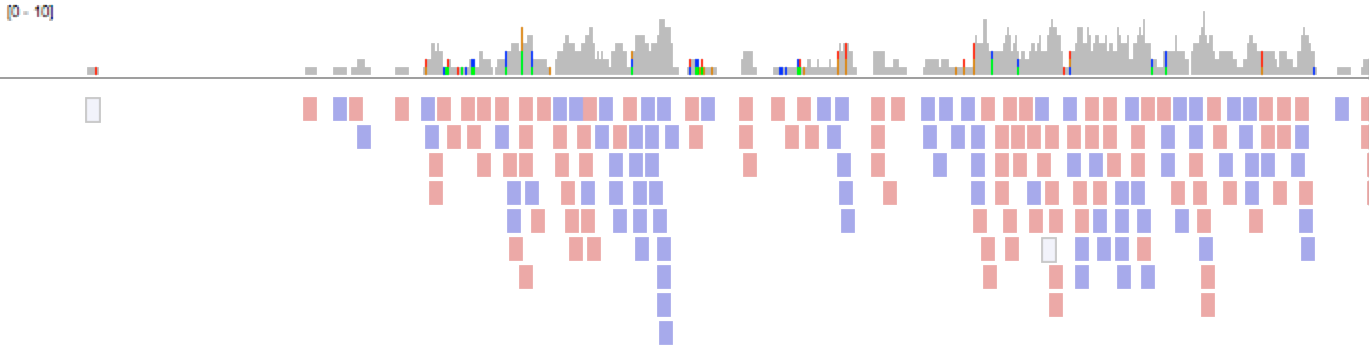
\includegraphics[width=\textwidth]{images/introduction/igv_panel_screenshot_k562_h3k4me3_WDTC1-transparentbcg.png}
    \caption{Integrative Genomics Viewer (IGV) \cite{Thorvaldsdottir:2012wy} screenshot of H3K4Me3 enrichment in the genetic region around the transcription starting site for gene \emph{WDTC1} (chr1:27,559,006-27,563,006) in cell type K562. The data was generated by ChIP-Sequencing in Broad institute and is available to download from ENCODE Project \cite{TheENCODEProjectConsortium:2004db}}
    \label{fig:igv_screen}
\end{figure}

Sequencing procedures generate millions of short reads of DNA that are aligned
to the reference genome. These alignments are stacked together to generate a
landscape of region enrichment over the whole genome.  Figure
\ref{fig:igv_screen} shows a sample of this landscape around the transcription
start site for gene \emph{WDTC1}. One can see the reads aligned to the genome
and the mark they form in the image.

ChIP-Seq can be used to study transcription factor binding sites of proteins
that interact with DNA, or can be used to study the chromatin within the DNA
itself. Chromatin is a combination of DNA and proteins that also lie within the
nucleus.  A major unit of a chromatin is a nucleosome, that consists of a
string of DNA wrapped around core histone proteins.  Histones are proteins
responsible for the compacting the DNA to fit inside the nucleus of a cell.
These proteins are acceptors for variety of modifications such as methylation
and acetylation of lysine (K) residues\cite{Fischle:2003tl}. These modifications
are often associated with DNA-based functions and such as transcription of
genes.  The histone modification mechanism is hypothesised to play a part in
these DNA-based functions by  "unravelling" the chromatin so it is more
accessible, and by recruiting non-histone proteins \cite{Kouzarides:2007ui}.

The size of the DNA raises a serious problem to the analysis of ChIP-Seq
results.  A variety of methods to identify regions of interest within the
dataset are available \cite{Park:2009wc}. These methods rely on \emph{peak
    calling} a statistical method of detecting regions in the genome that are
enriched significantly more than the background. One of such peak callers,
MACS, models the shift small shift between the reads on the strands that is
observed due to directionality of reads, adjusts the dataset according to this
model, and then models the  enrichment using a Poisson distribution
\cite{Zhang:2008wp}.

The enriched regions detected by peak callers (peaks) need to by analysed for
biological significance after they are identified. This is a challenging
problem due to a few reasons. Firstly, peaks tend to be of three different
types: sharp -- creating one high column of peak reads a few base pairs high;
broad -- significantly enriched regions spawning a long region of genome; and
mixed -- usually sharp peaks followed by a broad region\cite{Park:2009wc}.

Transcription factor binding site peaks are usually sharp. Broad and mixed
regions are common for histone modification analysis datasets. This project is mostly concerned
with histone modification datasets and therefore will study broad and mixed peaks.

\begin{figure}[p]
   \centering
   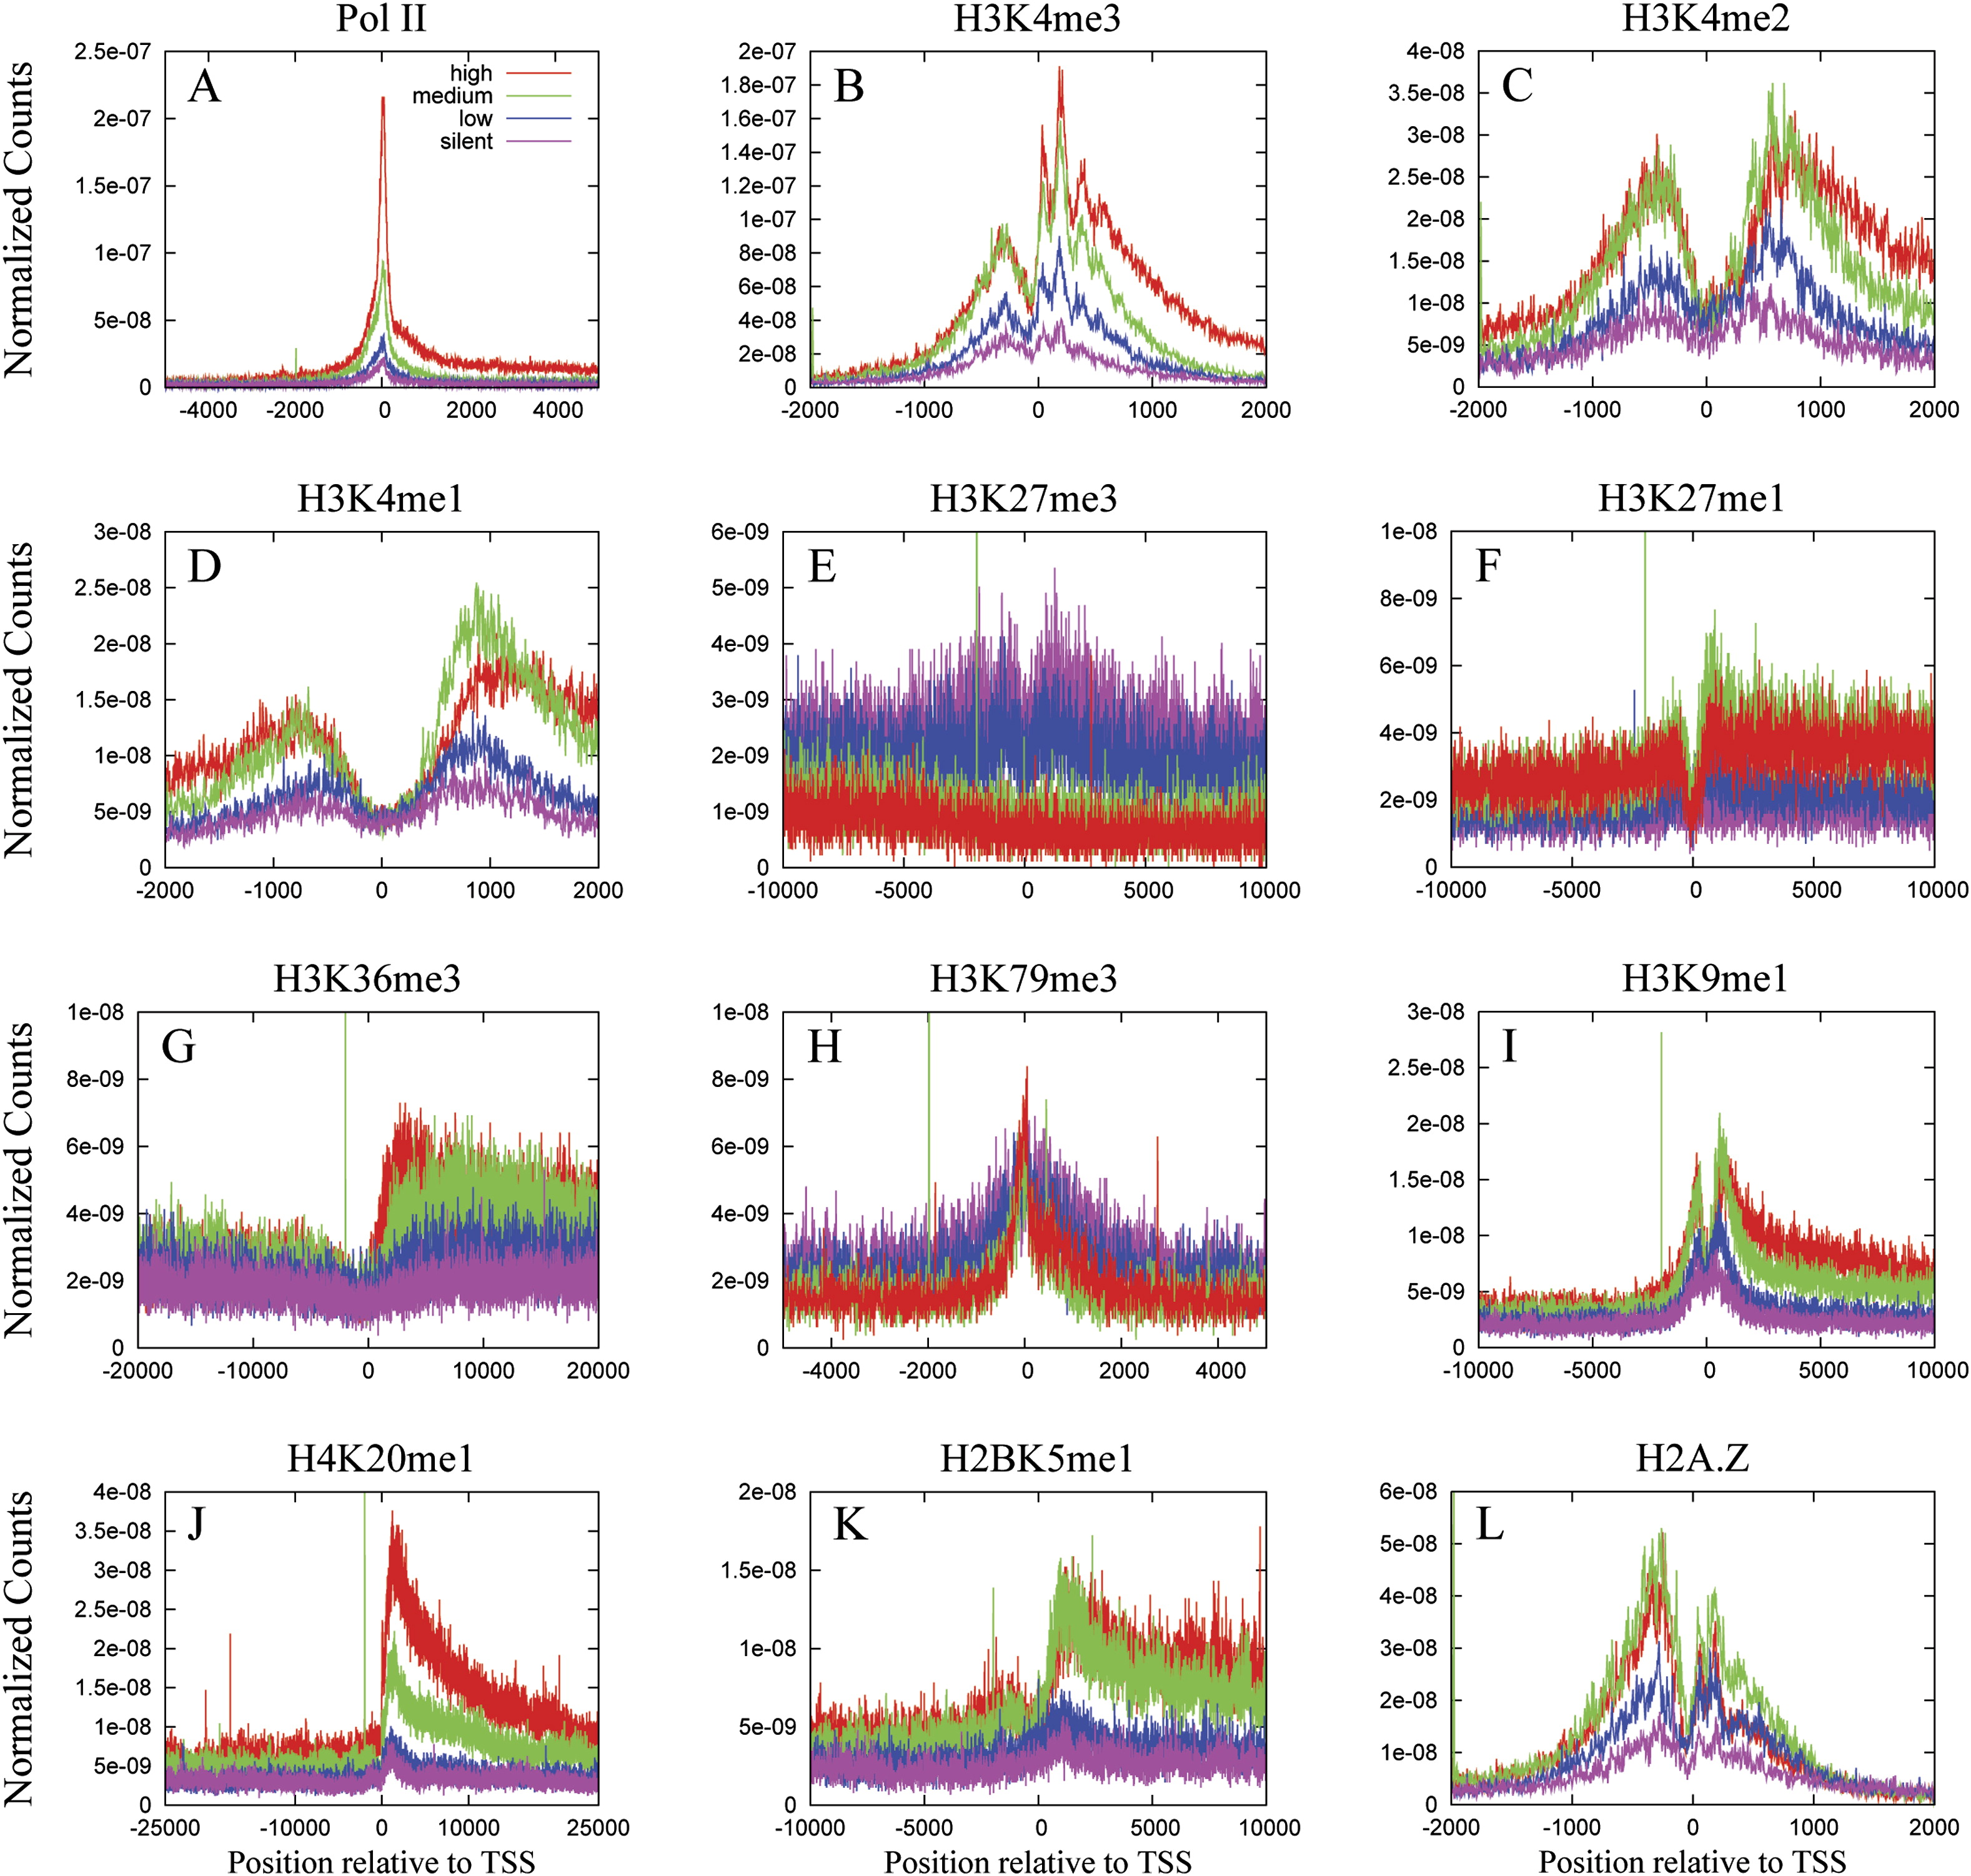
\includegraphics[width=\textwidth]{images/introduction/barski-histone-modifications-around-tss.jpeg}
   \caption{Profiles of the histone methylation indicated above each panel across the TSS for highly active, two stages of intermediately active and silent genes are shown.}
   \caption*{Reproduced from Cell, 129, Artem Barski, Suresh Cuddapah, Kairong Cui, Tae-Young Roh, Dustin E. Schones, Zhibin Wang, Gang Wei, Iouri Chepelev and Keji Zhao, High-Resolution Profiling of Histone Methylations in the Human Genome\cite{Barski:2007ww}, p. 826, Copyright 2007, with permission from Elsevier}
    \label{fig:barski_histone_profiles}
\end{figure}

%In [170]: lengths[lengths == lengths.median()].index[3]
%Out[170]: 'uc003okl.3'

%In [171]: lengths[lengths == lengths.median()].index[8]
%Out[171]: 'uc021uwd.1'

\begin{figure}
    \centering
    \begin{subfigure}[b]{\textwidth}
        \centering
        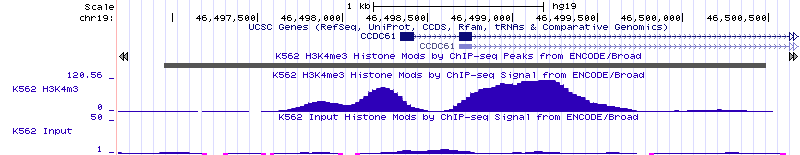
\includegraphics[width=\textwidth]{images/introduction/genome_browser_ccdc61.png}
        \caption{\emph{CCDC61}, chr19:46,496,682-46,500,682}
        \label{fig:genome_browser_ccdc61}
    \end{subfigure}
    ~
    \begin{subfigure}[b]{\textwidth}
        \centering
        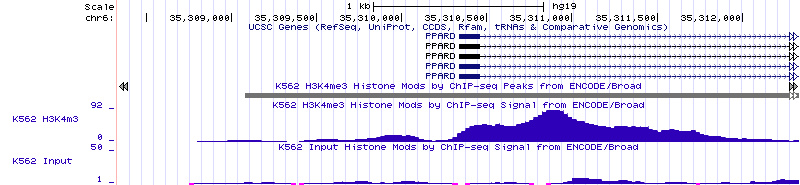
\includegraphics[width=\textwidth]{images/introduction/genome_browser_ppard.png}
        \caption{\emph{PPARD}, chr6:35,308,334-35,312,334}
        \label{fig:genome_browser_ppard}
    \end{subfigure}
    \caption{Genome-Browser screen-shot of H3K4Me3 marks for two different regions of the genome. The top track in each of the images shows locations of known genes. The first chart in each of the images is the H3K4Me3 signal registered from ChIP-seq experiments. The bottom track shows the control signal from the same experiment. Black line above the first chart marks regions that are thought to be significantly enriched.}
    \label{fig:different_marks}
\end{figure}

\begin{figure}[p]
    \centering 
    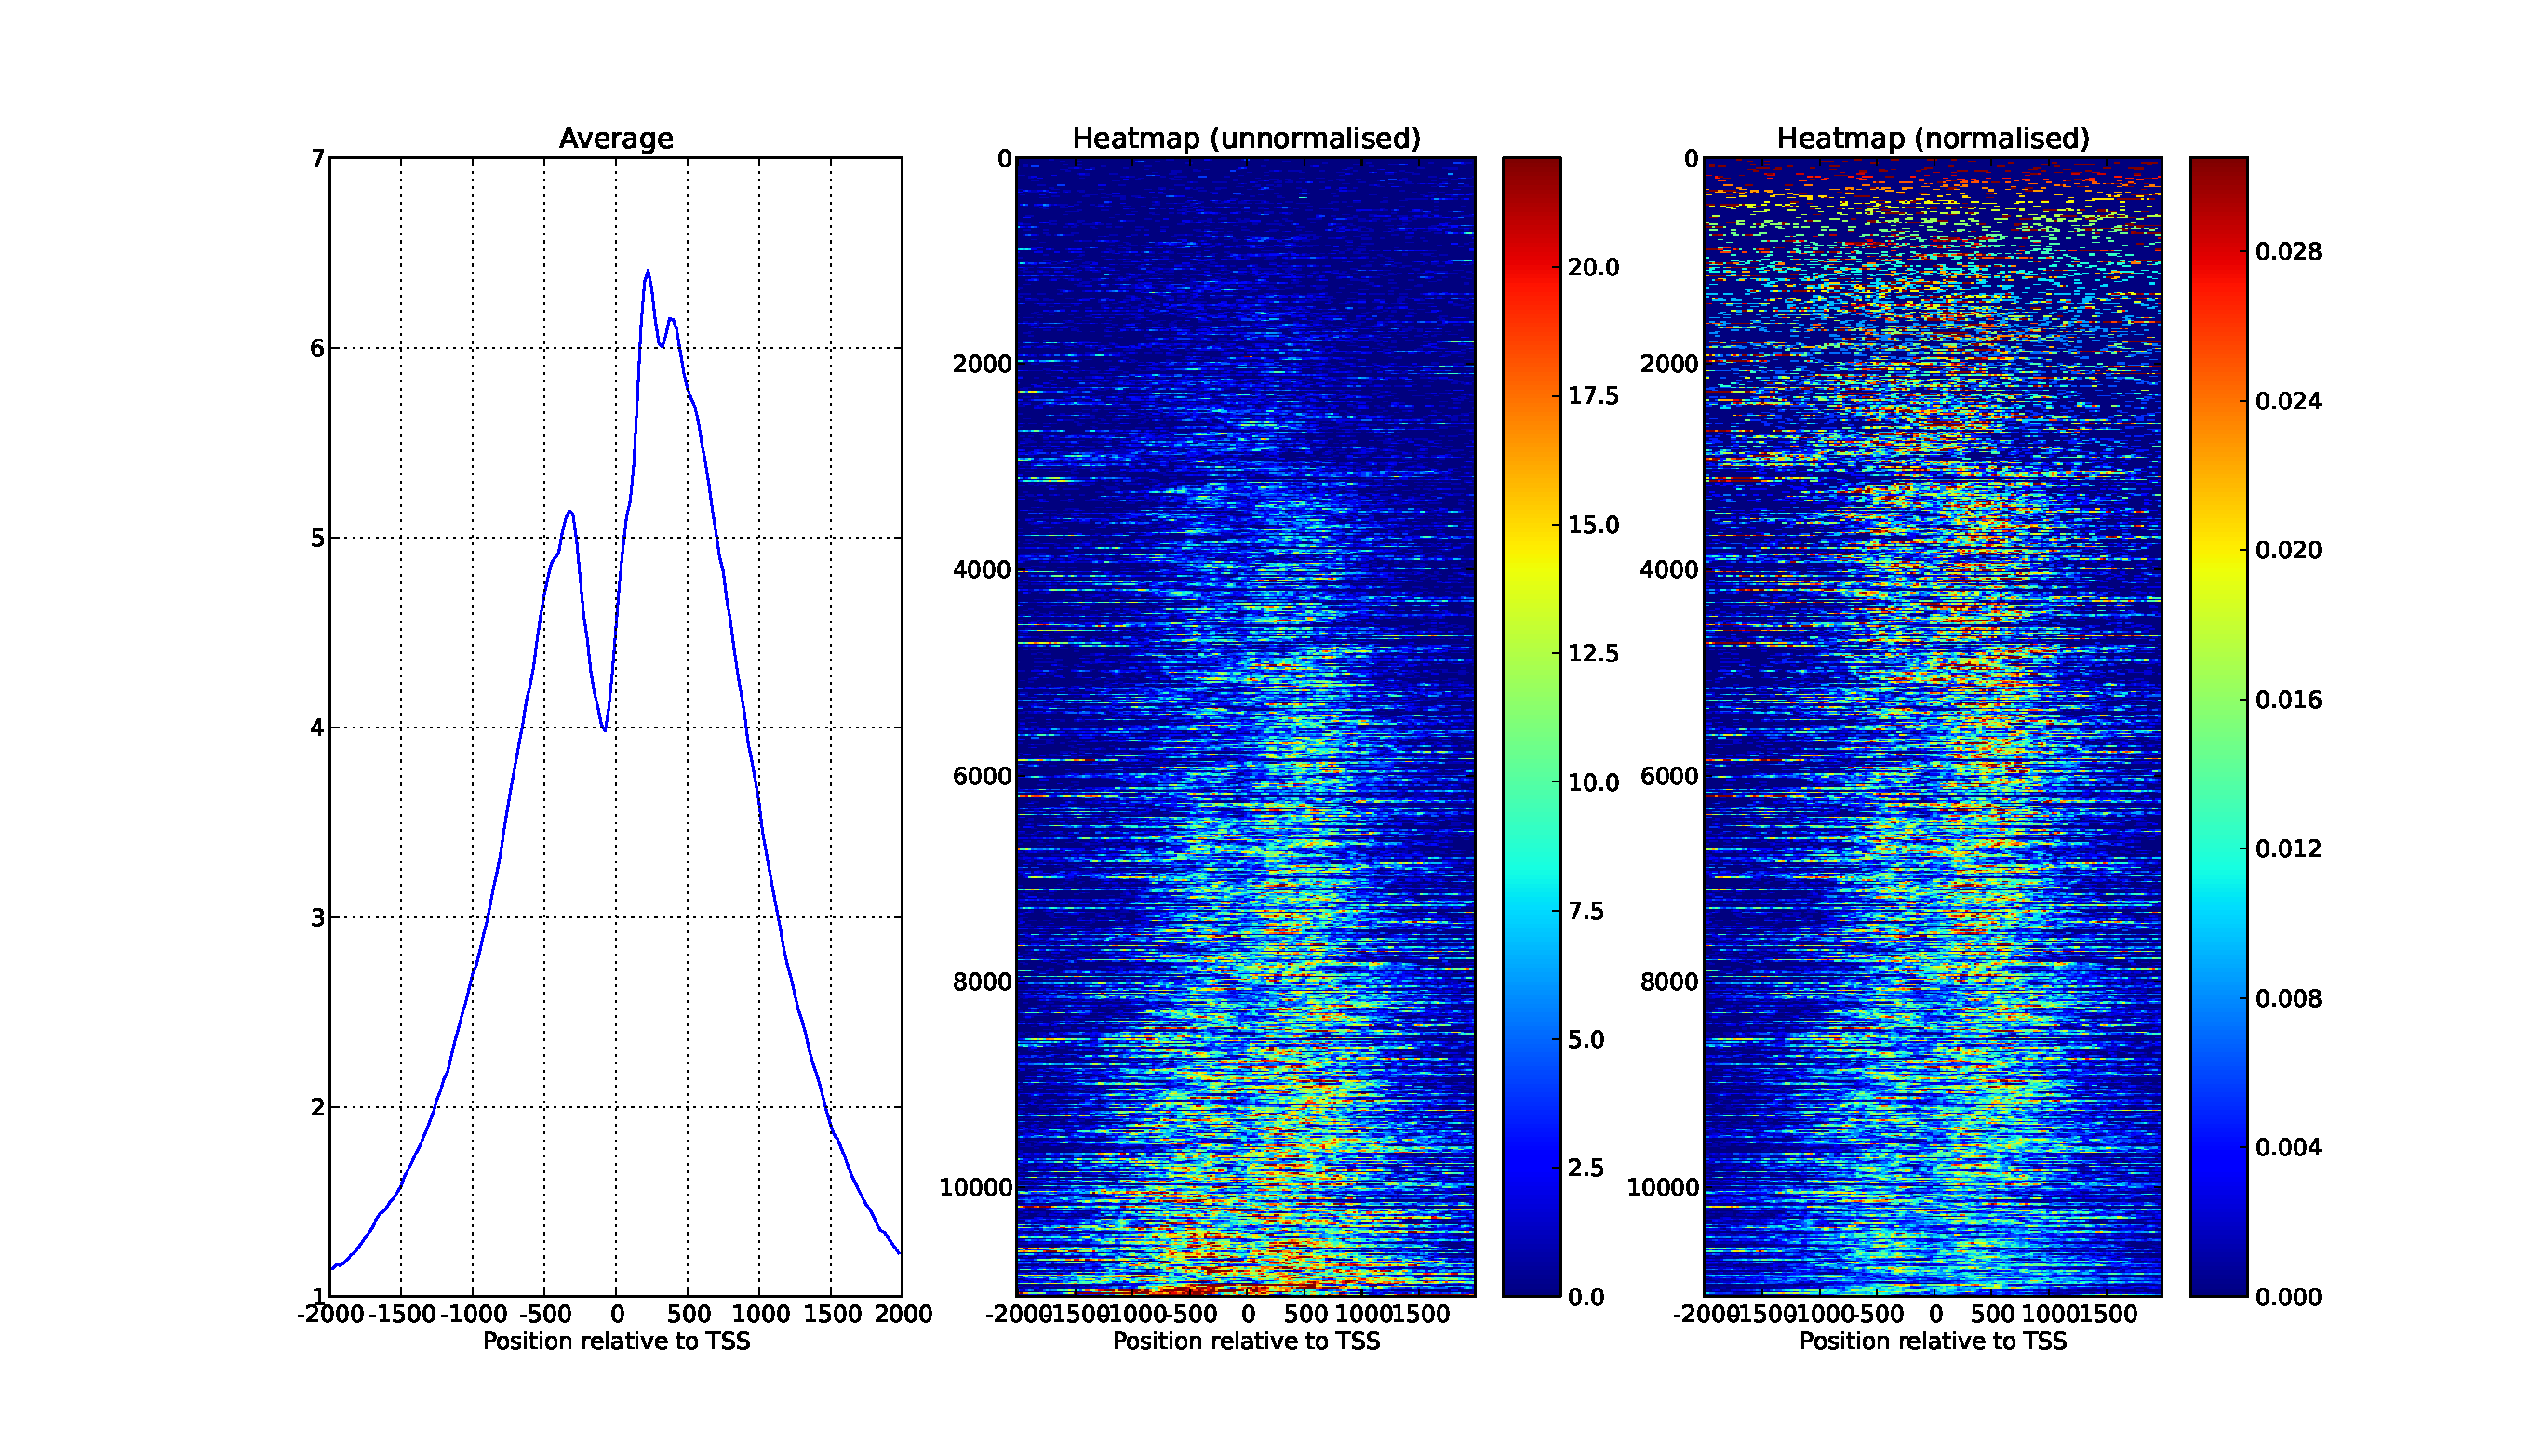
\includegraphics[width=\textwidth]{images/introduction/heatmap_k562-h3k4me3.eps}
    \caption{H3K4Me3 profile in cell type K562 around 11062 Transcription Start Sites of genes on positive strand. The figure shows average profile for the histone marks in the leftmost column. The middle column shows a heatmap of all the enrichment regions across these TSS, sorted by read count. The rightmost column shows the same regions displayed in the middle column normalised by the total number of read counts falling in the region as to compare the shapes of the marks on the same scale. One can see that the bimodal shape is clearly visible in the heatmaps, yet there is a lot of variability about the histone mark shapes in the dataset.}
    \label{fig:k562_positive_strand_heatmap}
\end{figure}

Artem Barski and colleagues have studied the profiles of ChIP-seq enrichments
for histone methylations across transcription start sites (TSS). Average
histone methylation profiles near Transcription Start Sites they have found are
shown in Figure \ref{fig:barski_histone_profiles}. One can see from this figure
that Histone 3 lysine 4 (often abbreviated H3K4) methylations form a bimodal
peak around transcription start site on average.  However, important
information about variance of data is lost when averaged.  For instance,
Histone 3 lysine 4 trimethylation (H3K4Me3) mark for TSS near gene
\emph{CCDC61} is very different to the H3K4Me3 mark around the TSS for gene
\emph{PPARD} as figure \ref{fig:different_marks} illustrates. In fact, the
latter mark, figure \ref{fig:genome_browser_ppard}, looks very diferent from
the typical mark obtained by averaging all marks. Figure
\ref{fig:k562_positive_strand_heatmap} plots a heatmap of a selection of
transcription start sites
\todo{Describe how the selection was obtained (TSSes on positive strand)}, 
showing that this variance is common on genome scale.

The assumption behind this project is that this variance encodes important
information. In other words, different histone marks may encode different
function. Evidence of this has been provided by previous research, e.g.
Heintzman et al., 2008 has used supervised learning approach to identify a
novel enhancer\cite{Heintzman:2007kea}. The first unsupervised method of
clustering chromatin signatures, \emph{ChromaSig}, has been developed in
2008\cite{Hon:2008wv}.  The downside of the algorithm described in this paper
is that \emph{ChromaSig} algorithm fixes the width of histone marks, even
though histone marks vary in their width significantly.  Furthermore, the
algorithm relies on on incrementally building histone modification patterns,
meaning that the algorithm is sensitive to the order in which these patterns
were processed as well as to the seed sequence.

A more recent paper describes
ChAT algorithm that takes a very similar approach to the one taken in this
project.  The paper uses dynamic programming measure similar to DTW to align
histone marks to each other \cite{Wang:2012cb}. This distance measure does not
require fixed-width windows and allows some slack to be incorporated by not
mapping a point on one sequence to some other point in the other sequence.
\emph{ChAT} then clusters these points using agglomerative clustering, and uses
significance threshold to divide the data into clusters. 

\section{Dynamic Time Warping}

This paper proposes the use of Dynamic Time Warping (DTW) distance for
clustering Histone Marks. Dynamic Time Warping is a Dynamic Programming
algorithm originating from Speech Recognition researchers. The algorithm
compares two distinct time series by arbitrarily stretching or compressing
(warping) the time axes. This time axis transformations allows the algorithm to
compare the sequences that vary in the time axis to be compared on the same
scale. For instance, think of a word that is spoken in a fast manner versus the
same word spoken slow. Even though the algorithm is designed for time series
analysis (therefore the name Dynamic \emph{Time} Warping), it can be used for
comparison of any sequences of any lengths. In case of histone marks data, the
algorithm would try to stretch or compact the DNA sequence to try and align the
histone marks as close as possible. 

The general case of algorithm as described in (Muller, 2007) \cite{Muller:2007bo} is described bellow.

Suppose we have two sequences $\mathbf{a} = a_1..a_n$ ($|\mathbf{a}| = n$) and $\mathbf{b} = b_1..b_m$ ($|\mathbf{b}| = m$).

We have a local distance measure, $d$ that measures the distance between two elements of the sequence, e.g. squared euclidean distance measure.

DTW aims to construct a warping path $\mathbf{p} = { (p_{1,0}, p_{1,1}), (p_{2,0}, p_{2,1}), ..., (p_{k,0}, p_{k, 1}) }$ that maps each point on the first sequence, specified as $p_{i,0}$ to a point on the second sequence, $p_{i,1}$. This warping path should be minimal in the sense that sum of the distances of all of the mapped points is minimal and the following three constraints should hold\cite{Muller:2007bo}:
\begin{enumerate}
\item \emph{Boundary Condition}: The path must start at the first point of sequence $\mathbf{a}$ and this point must be mapped to the first point of the second sequence: $p_1 = (1,1)$. Similarly, the final points of both sequences should be mapped to each other, and the path must end there: $p_k = (m, n).$ 
\item \emph{Monotonicity Condition}: The path must not move \emph{back in time}: 
    $p_{1,i} \le p_{2,i} \le p_{3,i} \le ... \le p_{k, i}$ for both $i=0$ and $i=1$.
\item \emph{Step Size Condition}: At each step the path must either map the same point on one sequence to the next point on another sequence, or map next points on both sequences together, mathematically:
    $p_{i+1} - p_{i} \in \{(0,1), (1,0), (1,1)\}$ for all $i < k$.
\end{enumerate}

One can solve the problem of finding the minimal mapped distance in $O(nm)$ time by applying dynamic programming techniques. We construct a $n \times m$ matrix $\mathbf{D}$ where each entry $D_{i,j}$ will contain a minimal (warped) distance of matching first $i$ components of the first sequence, $a_1..a_i$, to first $j$ elements of the second sequence, $b_1..b_j$. The first component of the matrix, $D_{1,1}$ is initialised to the distance between the first components of the two sequences, $d(a_1, b_1)$ as specified by the boundary condition.

The matrix is then filled row by row, according to the following recursive equation:
$$D_{i,j} = d(a_i, b_j) + min(D_{i-1, j}, D_{i, j-1}, D_{i,j})$$

In the end, the column $D_{n,m}$ holds the minimal warped distance between two series.

If the minimal warping path is needed, it can be traced back by following the recursive relation backwards from $D_{i,j}$.

Figure \ref{fig:dtw_alignment_example} shows DTW alignment for the H3K4Me3
marks in figure \ref{fig:different_marks}. As one can see from this image, DTW
algorithm maps the first forty bins (1000 base pairs) from the first sequence to
the first bin of the second sequence. This is roughly equivalent of cutting the first 40 bins
of the first sequence off. Visually inspecting the sequences, cutting the first 40 bins off makes the patterns much closer than they were before.

\todo{Look up why the numbers are different in genome browser shots and in the DTW.}

\begin{figure}[t,b]
    \centering
    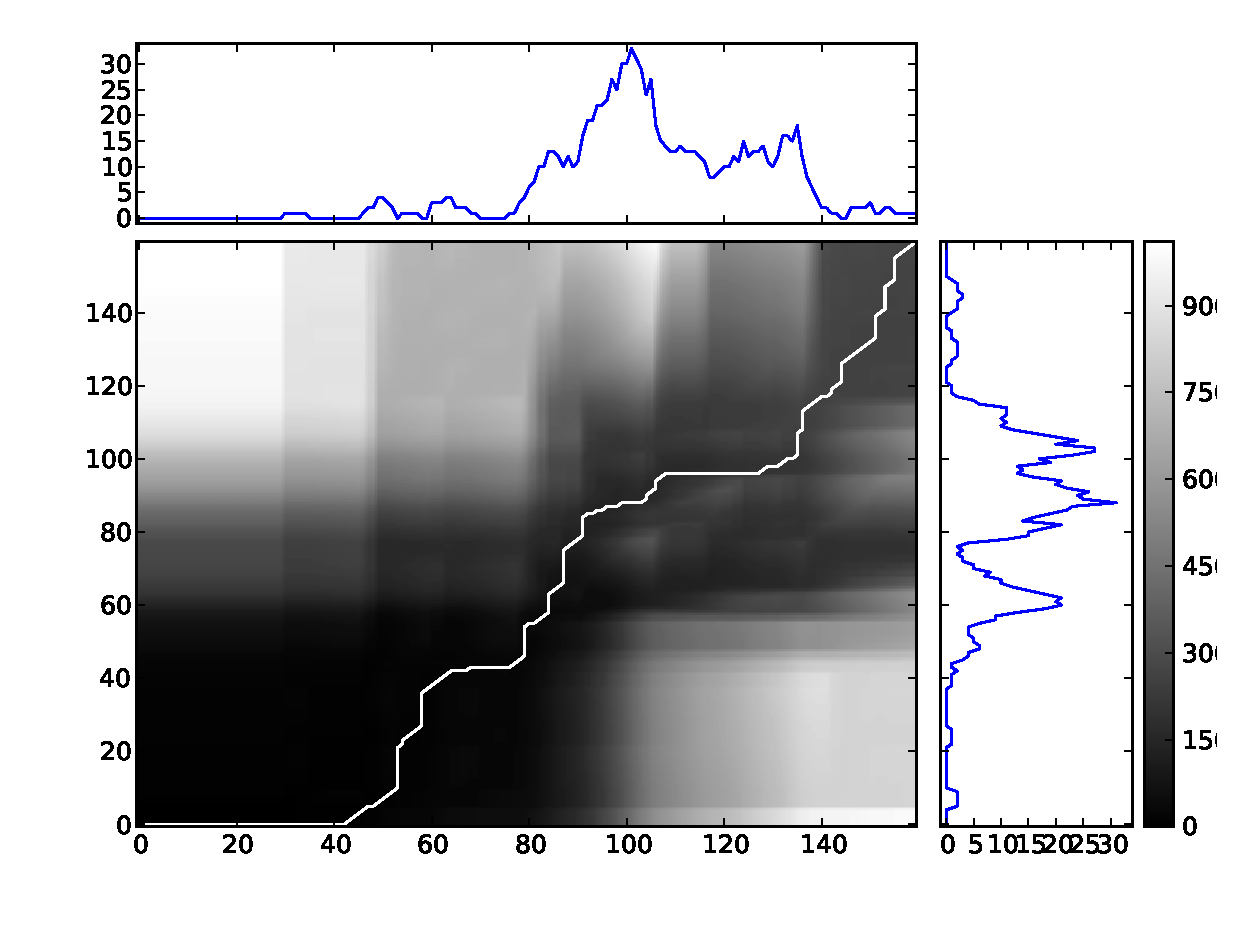
\includegraphics[width=\textwidth]{images/introduction/dtw_dist_uc003okl_3_uc021uwd_1.eps}
    \caption{Accumulated cost matrix $\mathbf{D}$ (heatmap) and the optimal
        warping path (white line) for DTW alignment of regions in
        \ref{fig:different_marks}. The numbers on x and y axes of the heatmap
        represent 160 bins that are 25 base pairs wide where the data was aggregated to.
        }
    \label{fig:dtw_alignment_example}
\end{figure}

\subsection{Global constraints on Dynamic Time Warping}

Even thought the \emph{cutting off} of the first 40 base pairs, reduces the
total distance in the example shown in \ref{fig:dtw_alignment_example}, this
might not necessarily be what we want to do. In this particular example, we
may want to penalise the mark for having a long unexpressed region in the
beginning.  This could be done by constricting the set of paths DTW considers.
If mapping the first 40 bins to the same point was not allowed by this
restriction, the algorithm would be forced to look for alternative and thus more
expensive paths.  

The two most commonly used global constraints on DTW are the Sakoe \& Chiba
Band\cite{Sakoe:1978ta} and Itakura Parallelogram\cite{Itakura:1975jh}. 

Sakoe \& Chiba band forces each point in the path to satisfy $|i-j| <= k$ for
some $k$. Roughly speaking, parameter $k$ specifies how much the time axis
could be squeezed. The assumption behind this is that in case of a perfect match 
the time axis does not need to be stretched and the optimal warping path runs over the diagonal.
The parameter $k$ allows slight deviations from this diagonal to only allow close matches between two series.
This parameter needs to be estimated from the dataset,
even though value of 10\% of the sequence length has been used
historically\cite{Ratanamahatana:2004wu}. It is important to note that Sakoe \&
Chiba band does not work with sequences whose lengths differ by more than k as the last point on the path, $(n,m)$, will not satisfy the global constraint. 
Ratanamahatana \& Keogh argued that this is not a serious issue as
the sequences can be rescaled without detrimental effects, however research by
Henniger and Muller (2007)\cite{Henniger:2007us} has found evidence of
detrimental effects of rescaling, therefore a good thought must be put into implementation
of this constraint for sequences of different lengths.

Another kind of global constraint, Itakura Paralellogram, constrains the
warping paths more near the ends of the sequences more than in the middle --
the cost matrix forms a parallelogram. This constraint does not require a parameter to be set, but is used less often than Sakoe \& Chiba band, most likely because the latter is much simpler to implement.

\begin{figure}[t,b]
    \centering
    \begin{subfigure}{\textwidth}
        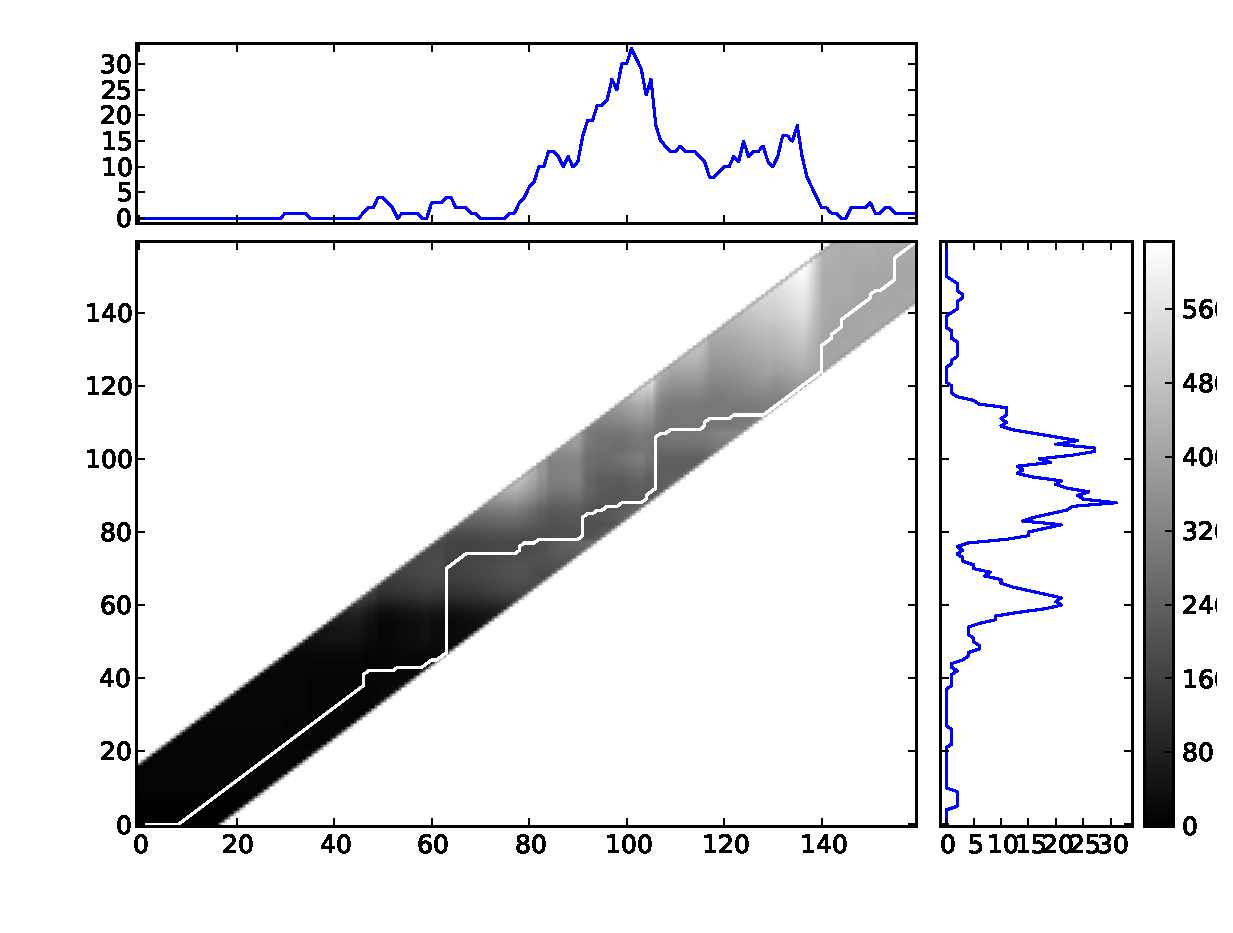
\includegraphics[width=\textwidth]{images/introduction/dtw_dist_uc003okl_3_uc021uwd_1_sakoe_chiba_16.eps}
        \caption{Sakoe \& Chiba band (10\%)}
        \label{fig:dtw_alignment_example_sc}
    \end{subfigure}
    ~
    \begin{subfigure}{\textwidth}
        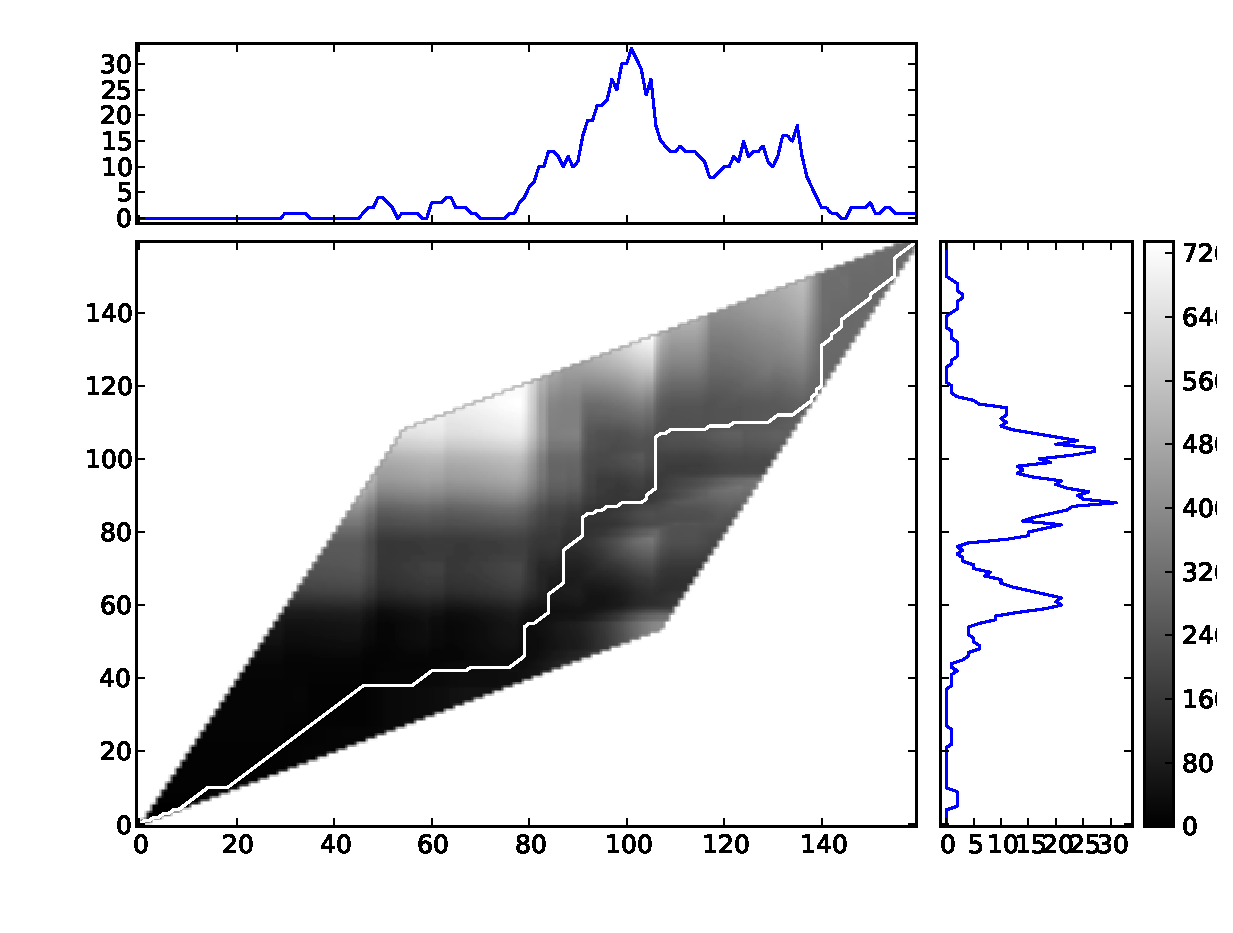
\includegraphics[width=\textwidth]{images/introduction/dtw_dist_uc003okl_3_uc021uwd_1_itakura.eps}
        \caption{Itakura Parallelogram}
        \label{fig:dtw_alignment_example_itakura}
    \end{subfigure}
    \caption{The sequences in the example in \ref{fig:dtw_alignment_example} DTW-aligned with global constraints in place}
    \label{fig:dtw_alignment_example_constrained}
\end{figure}

Figure \ref{fig:dtw_alignment_example_constrained} illustrates these concepts
of constraining the DTW over the same sequences used in figure
\ref{fig:dtw_alignment_example}. Both of the constraints stop the algorithm
from truncating the first forty bins and make it take the more expensive path
instead.

It also must be mentioned that global constraints give a computational
advantage for the algorithm as well. For instance, Sakoe \& Chiba band with
parameter k reduces the time complexity to $O(k \times max(m, n))$ as only the
distances within the band need to be evaluated. Since, $k \ll m,n$ in most
cases, the reduction is significant. In fact, in some 
cases DTW with Sakoe \& Chiba constraint is used to calculate the lower band on
DTW distance, before computing the full DTW distance, as to prune a large part of 
comparisons away \cite{Ratanamahatana:2004wu}.

\subsection{Properties of DTW Distance}

It is trivial to see that Dynamic Time Warping distance is symmetric, provided
that the local distance measure is symmetric. However, the DTW distance does
not satisfy the triangle inequality, even when the local distance measure
does\cite{Muller:2007bo,Niennattrakul:2007wv}.

This has some implications to clustering -- no tractable method to find the
sequence that minimises the distance to all other sequences for a set of DTW
sequences is known. That means that centroid based clustering methods must rely
on approximations. A few possible approaches are reviewed in
\cite{Niennattrakul:2007wv,Petitjean:2011bq}.  Hierarchical clustering is also
affected by this. Since the triangle equality is not satisfied, agglomerative
clustering with single-link linkages suffers from a phenomenon known as
\emph{chaining} where whole dataset gets linked to the same cluster of data one
link at a time. Fortunately, Shoji Hirano and Shusaku Tsumoto have shown that
complete-linkage criterion is not prone to this\cite{Hirano:2005wh}. 

\section{Work done so far}
To this date the following work has been completed:
\begin{enumerate}
\item Routines for processing the ChIP-Seq datasets for reading BED files and extracting the data from BAM files were implemented in Python.
\item MLPY's\cite{Albanese:2012vf} implementation of DTW was extended by efficient
    implementation of Sakoe \& Chiba band and Itakura paralellogram constraints in C.
    This implementation is ready to be submitted to project authors for official inclusion.
\item Prototype for hierarchical clustering using DTW distance implemented and efficiently uses all CPUs available in the machine.
\item Prototype routines for plotting the chip-seq data have been implemented in Python.
\end{enumerate}

\section{Work planned}
\begin{enumerate}
    \item The current prototypes need to be refactored, documented and packaged to a working package that could later be published.
    \item An automatic test or a GUI tool needs to be developed that would cut the dendrogram obtained by agglomerative clustering.
    \item The algorithm needs to be extended to handle multiple-dimension data;
    \item Finally, critical evaluation of the performance of the algorithm needs to be done, that would include downstream analysis, e.g. by comparing it to gene ontology data\cite{Botstein:2000ja}.
\end{enumerate}

\bibliographystyle{unsrt}
\bibliography{papers2}

\end{document}
